\documentclass{beamer}
\usepackage[utf8]{inputenc}
\usepackage[T1]{fontenc}
\usepackage{lmodern}
\usepackage[scaled=.95]{libertine}
\usepackage{algorithm}
\usepackage{algorithmic}
\usepackage{subfigure}
%\usepackage{picins}%mix figures and text together
\usepackage{picinpar} 

%\usepackage[loosequotes]{MinionPro}
%\usepackage{MnSymbol}
%\pdfmapfile{+MinionPro.map}
\bibliographystyle{plain}
\usepackage[orientation=portrait,size=a0,scale=1.9]{beamerposter}

\usepackage{fixltx2e}
\usepackage{graphicx}
\usepackage{tabularx,multirow,booktabs}
\usepackage{relsize}
\setlength{\abovecaptionskip}{0pt}
\newcommand\LI[1]{\textrm{`#1'}}
\newcommand\acronym[1]{\textsmaller{\MakeUppercase{#1}}}

\usetheme{LLT-poster}
\usecolortheme{ComingClean}
\footimage{}%\includegraphics[width=.35\textwidth]{authors}}

\usepackage{tikz}

\title{An Efficient Online Event Detection Method for Microblogs via User Modeling}
\author[huangwaleking\string@gmail.com \hspace{.1em} \{pekingchenwei,tjwang\}@pku.edu.cn \hspace{.1em}citlmzhang@163.com]{Weijing \textsc{Huang} \and Wei \textsc{Chen} \and Lamei \textsc{Zhang} \and Tengjiao \textsc{Wang}}
\institute{\raisebox{-.2ex}{EECS, Peking University, Beijing}}
\date{}
\begin{document}
\begin{frame}
%\vskip-1ex
\begin{columns}[T]
\begin{column}{.46\textwidth}
\parbox[t][1200mm]{\textwidth}{
\begin{block}{Motivation}
\begin{itemize}
\item Detecting events in microblogs is important but still challenging.
        \begin{itemize}
                \item Tweet stream is a mixture of \textbf{user interests} and \textbf{external events}, it's difficult to distinguish them.
                \item Existing methods are ineffective since they ignore user interests or only model interests and events on a fixed dataset without scalability.
        \end{itemize}
\item We introduce an online learning model \textit{User Modeling Based Interest and Event Topic Model} (UMIETM).
        \begin{itemize}
                \item exploiting user profile to discover events by filtering out user interest-related tweets; treating the arriving data as stream and run the detection in online learning style.
        \end{itemize}
\end{itemize}
\end{block}


\begin{block}{Relationship between Profile and User Interests }
\begin{itemize}
        \item User profile is highly correlated to user's interests.
\end{itemize}
\begin{figure}[H]
        \centering
        \label{fig:profile} %% label for entire figure
        \subfigure[\tiny{Andrew Ng (Computer Scientist)}]{
                \label{fig:profile:c} %% label for first subfigure
                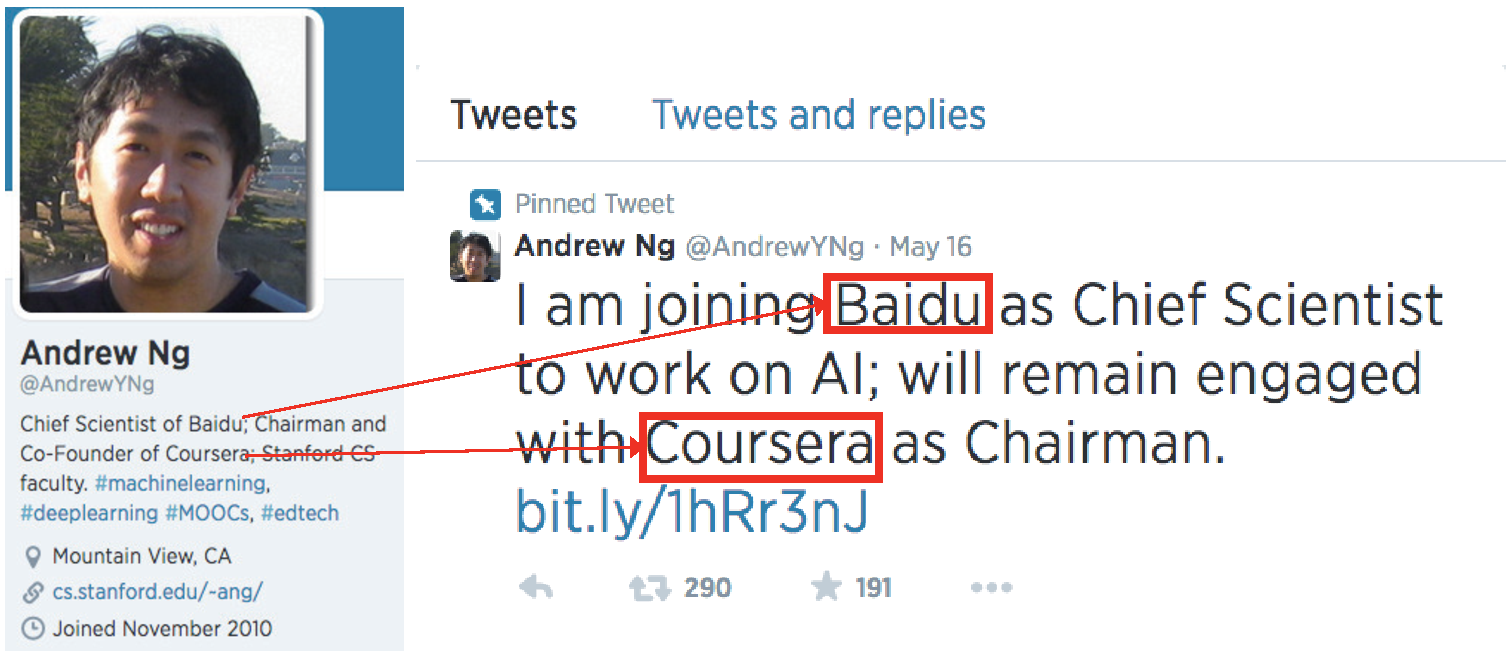
\includegraphics[height=8.5cm]{img/andrewNg.pdf}
        }  
        \subfigure[\tiny{Van Persie (Soccer Player)}]{
                \label{fig:profile:d} %% label for second subfigure
                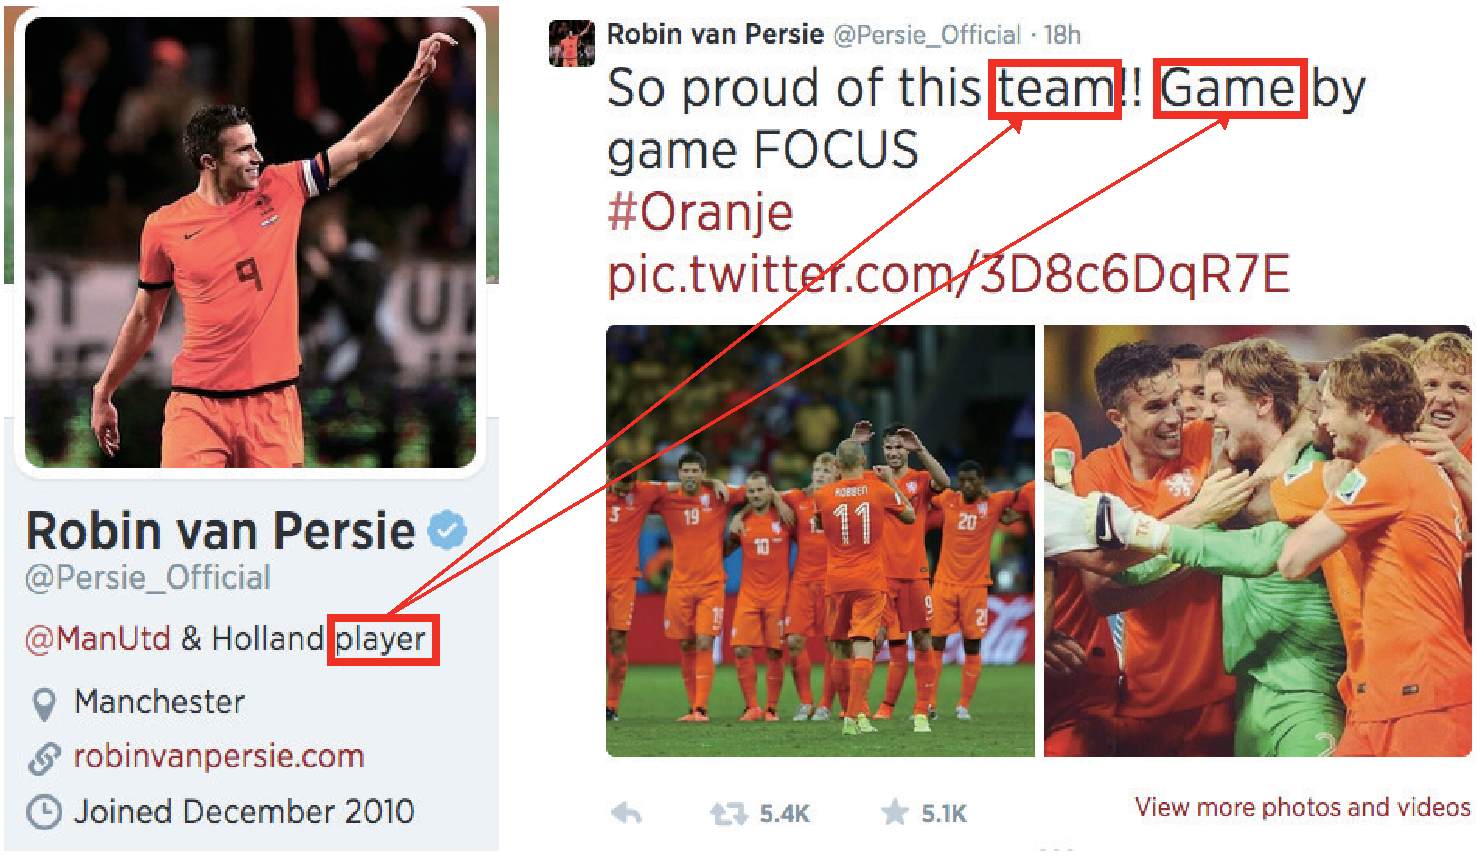
\includegraphics[height=8.5cm]{img/robinVanPersie.pdf}
        } 
%        \caption{\small{Illustration of the relationship between user profile and user interests}} 
\end{figure}
\begin{itemize}
\item Users who have similar user profiles also have similar interests.
        \begin{itemize}
                \item 46.2\% \#MachineLearning users also choose \#DataMining tag in their profiles.
        \end{itemize}
\item Users' interests can be enriched by followee's profiles.
        \begin{itemize}
                \item e.g. Biz Stone (\textit{Co-founder of Twitter, Medium, and now Co-founder and CEO of Askjelly.com}) follows 60 founders, 27 CEOs, 21 Google related, and 9 medium related accounts, etc. 
        \end{itemize}
\end{itemize}

%\begin{table}
%\centering
%\caption{\scriptsize{Word Clouds of tweets generated by users who have the specific user profile}}
%\scalebox{1.0}{
%\begin{tabular}{|l|c|c|c|c|c|c|}
%        \hline
%        \tiny{\#Buddhist} & \tiny{\#TOEFL} & \tiny{\#DataMinig} & \tiny{\#MachineLearning} & \tiny{\#PatternRecognization} & \tiny{\#Jewelry} & \tiny{\#Racing}\\
%        \hline
%        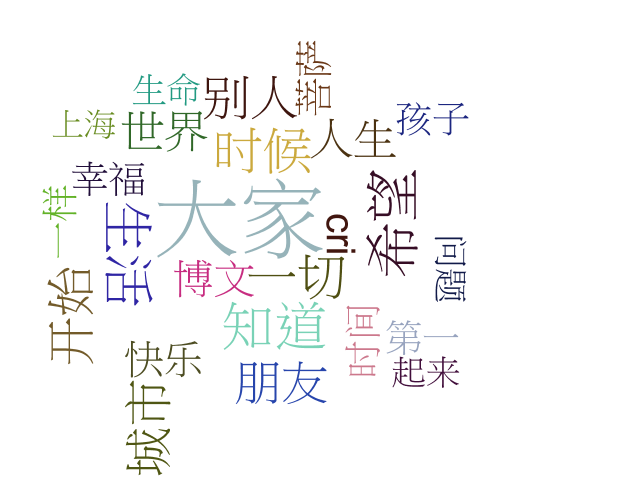
\includegraphics[width=.11\textwidth]{img/buddhist} & 
%        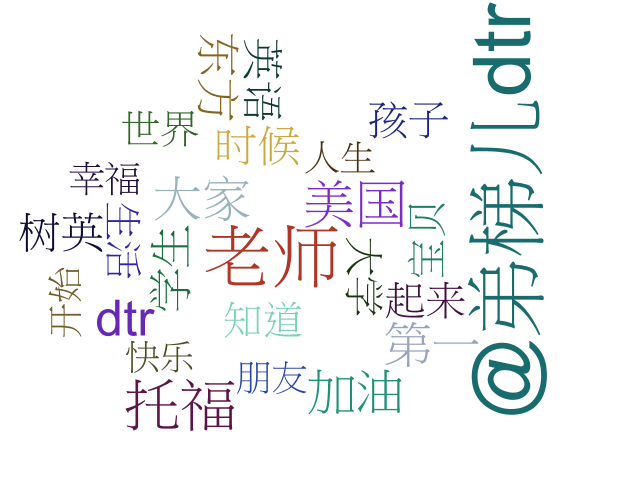
\includegraphics[width=.11\textwidth]{img/TOEFL} & 
%        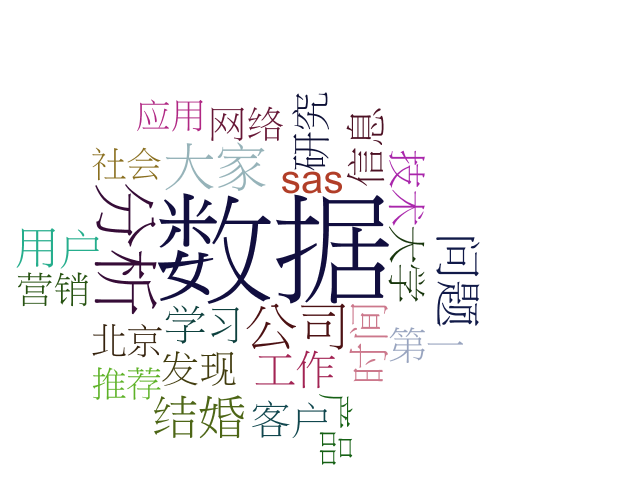
\includegraphics[width=.11\textwidth]{img/DataMining}&
%       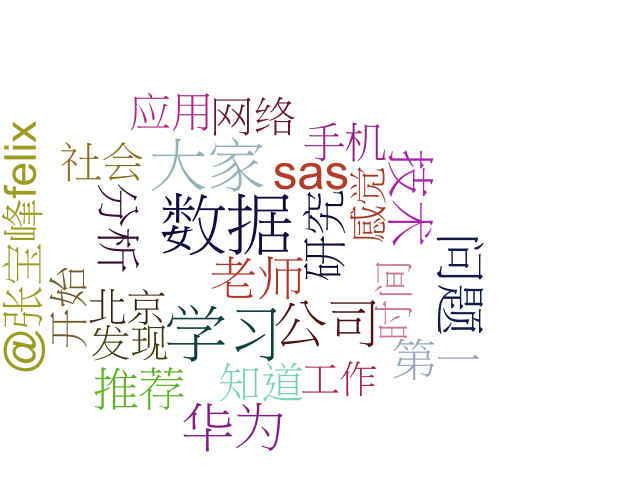
\includegraphics[width=.11\textwidth]{img/MachineLearning}&
%        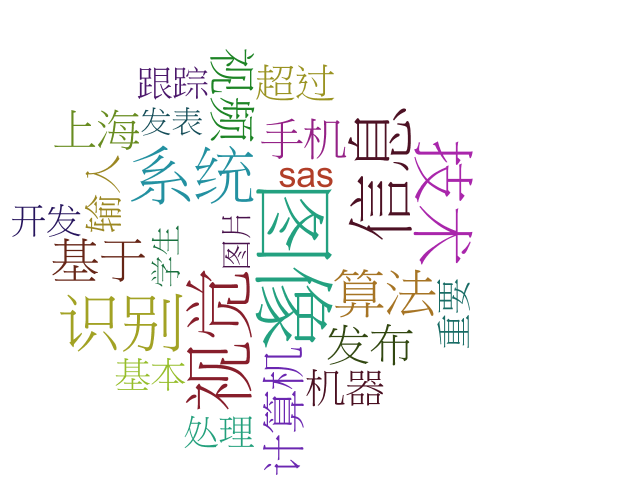
\includegraphics[width=.11\textwidth]{img/PatternRecognization}&
%        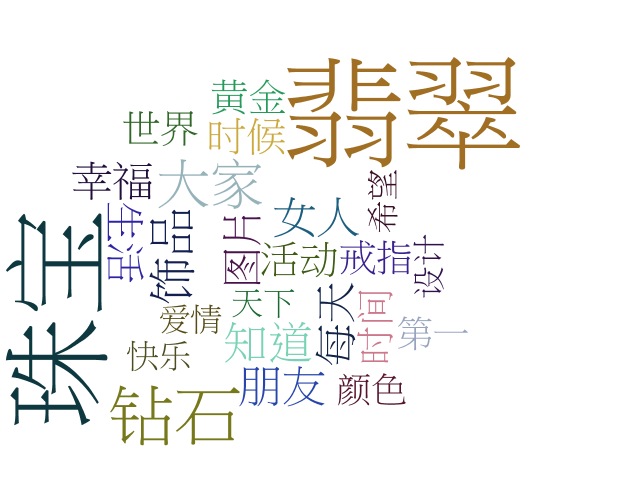
\includegraphics[width=.11\textwidth]{img/Jewelry}&
%        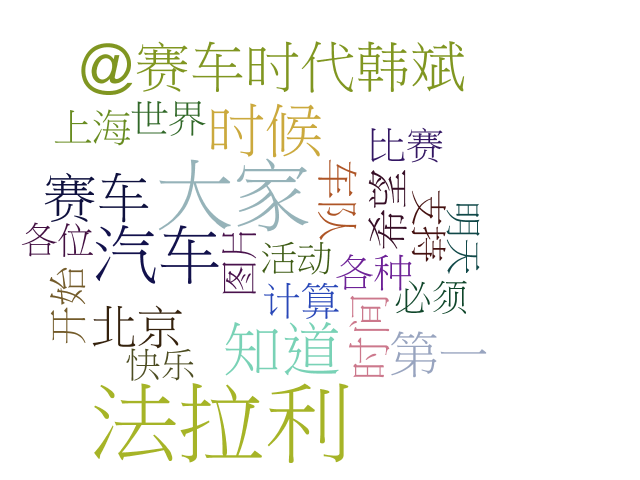
\includegraphics[width=.11\textwidth]{img/Racing}\\
%        \hline
%\end{tabular}
%}
%\end{table}     

\end{block}

\begin{block}{User Modeling Based Interest and Event Topic Model}
\begin{itemize}
\item Main idea 
        \begin{itemize}
                \item User and their followees' profiles are more stable to reflect user's interests than tweets; external events draw global attention in short time.
        \end{itemize}
	\begin{figure}
		\centering
		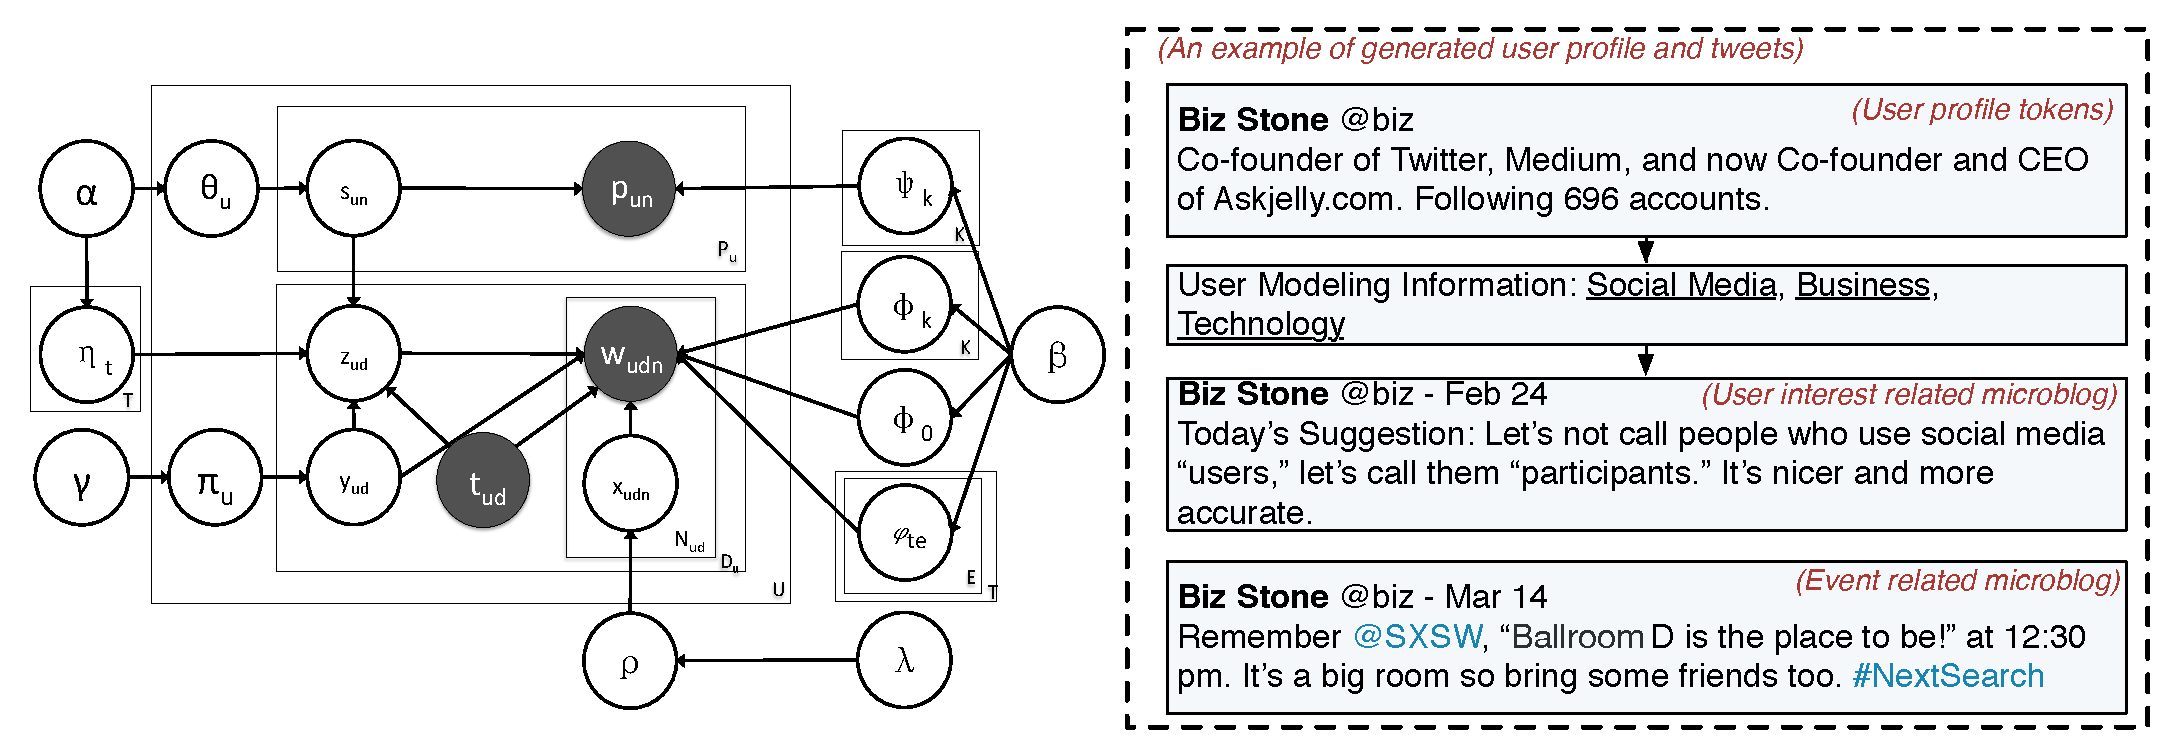
\includegraphics[height=12.5cm]{img/model.pdf}
%	\caption{Illustration of UPIETM}
		\label{fig:Illustration of UPIETM}
	\end{figure} 

\end{itemize}
                \begin{itemize}
                        \item generative process
                        \begin{itemize}
                                \item \footnotesize{user generates hidden profile topic \(s_{un}\) from user-interest distribution \(\theta_u\), then generates profile token \(p_{un}\) from multinomial distribution \(\psi_{s_{un}}\).}
                                \item \footnotesize{user decides to post interest-related tweet or event-related tweet according to switcher \(y_{ud}\).}
                                \item \footnotesize{if \(y_{ud}=0\), generates tweet's hidden topic \(z_{ud}\) from user's profile hidden topic \(\{s_{u1},\cdots,s_{un}\} \)uniformly, then generates tweet tokens from word-interest distribution \(\phi_{z_{ud}}\).}
                                \item \footnotesize{if \(y_{ud}=1\), generates tweet's hidden topic \(z_{ud}\) from event-time window distribution \(\eta_t\), then generates tweet tokens from word-event distribution \(\varphi_{t,z_{ud}}\).}
                        \end{itemize}
                \end{itemize}

\end{block}

}
\end{column}

\begin{column}{.46\textwidth}
\parbox[t][1200mm]{\textwidth}{

\begin{block}{Online Learning}
\begin{itemize}
\item Gibbs Sampling
	\begin{itemize}
	\item 1st phase: sample user profile's hidden topic \(s_{un}\).
	\item 2nd phase: joint sample tweet's hidden topic \(z_{ud}\) and \(y_{ud}\).
	\end{itemize}
\item Batch Learning is Expensive: \(O(I_1 K|P|+I_2 (K+E)|W|)\)
	\begin{itemize}
	\item \scriptsize{\(I_1\): iteration number of first phase sampling.}
	\item \scriptsize{\(I_2\): iteration number of second phase sampling.}
	\item \scriptsize{\(K\), \(E\): number of user interest related topics and number events in each time window.}
	\item \scriptsize{\(|P|\):  number of total user profile tokens; \(|W|\): number of total tweet tokens.}
	\end{itemize}
\item Online Learning
\begin{itemize}
\item Reuse the word-topic distribution in last time window
\item Smoothing for new words 
\begin{figure}[H]
        \centering
        \label{fig:subfig} %% label for entire figure
        \subfigure[online processing]{
                \label{fig:subfig:a} %% label for first subfigure
                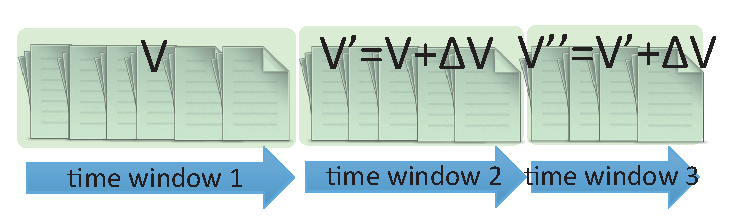
\includegraphics[height=4.3cm]{img/stream1.pdf}
        }  
        \subfigure[smoothing for new words]{
                \label{fig:subfig:b} %% label for second subfigure
                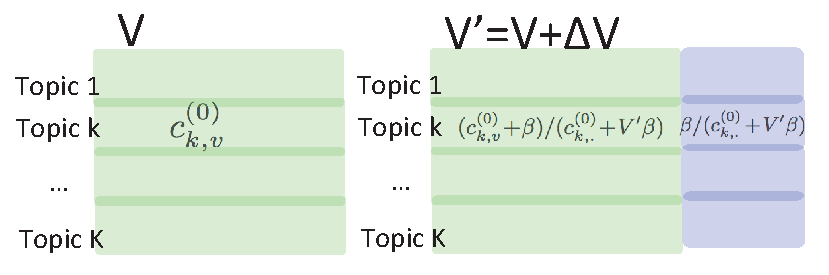
\includegraphics[height=4.3cm]{img/stream2.pdf}
        } \hspace{1in}
%        \caption{\footnotesize{Illustration on how to reuse the word-topic distribution in online style}}
\end{figure}
\item Complexity: \(O(I_1 K|P|+I_2 (K+E)|W_t|)\), where \(|W_t|\ll |W| \)

\end{itemize}

\end{itemize}
\end{block}

\begin{block}{Experiments}
\begin{itemize}
	\item Weibo Dataset
        \begin{columns}
                \begin{column}{.55\textwidth}
                        \begin{itemize}
                                \begin{itemize}
                                        \item \footnotesize{from Jan 2012 to Dec 2012}
                                        \item\footnotesize{split dataset by week}
                                        \item \footnotesize{segment Chinese words}
                                        \item \footnotesize{remove stop words, low freqency words}
                                        \item \footnotesize{remove tweets whose token number is less than 3}
                                \end{itemize}
                        \end{itemize}
                \end{column}
                \begin{column}{.45\textwidth}
                        \begin{table}
                                \centering
                                \caption{\scriptsize{statistics of processed dataset}}
                                \scalebox{0.44}{
                                        \begin{tabular}{|c|r|r|r|r|} \hline
                                         & \#user  & \#profile token & \#tweet & \#tweet token\\ \hline
                                        whole year& 252,369&  1,470,080 & 16,421,167 & 251,686,571\\ \hline
                                        week1 & 9,785 &  73,307& 31,503 & 440,217\\ \hline
                                        week2 & 29,721 & 222,280 & 242,554 & 3,679,979\\ \hline
                                        week3 & 30,891 & 231,042& 254,698 & 3,881,633\\ \hline
                                        \(\cdots\) & \(\cdots\)& \(\cdots\)& \(\cdots\)& \(\cdots\)\\ \hline
                                        \end{tabular}
                                }
                                \label{statisticsOfDataset}
                        \end{table}
                \end{column}
        \end{columns}
	\item Effectiveness
\begin{itemize}
\item Example events detected by UMIETM
\begin{table}[]
\centering
\label{fig:event}
\scalebox{0.6}{
\begin{tabular}{|c|l|l|}
\hline
\begin{tabular}[c]{@{}c@{}}Time \\ window\end{tabular} & \multicolumn{1}{c|}{Top words of example events} & \multicolumn{1}{c|}{Example events} \\ \hline
\multirow{2}{*}{\begin{tabular}[c]{@{}c@{}}The first \\ week of \\ 2012\end{tabular}} & \begin{tabular}[c]{@{}l@{}}Japan, earthquake, occur, the first day, \\ January, 7.0, 2012\end{tabular} & \begin{tabular}[c]{@{}l@{}}In January 1 of 2012, a magnitude-7 \\ earthquake occurred in Japan.\end{tabular} \\ \cline{2-3} 
 & \begin{tabular}[c]{@{}l@{}}New, year, happy, 2012, New Year’s \\ Day, healthy, blessing, happiness\end{tabular} & \begin{tabular}[c]{@{}l@{}}Everyone bless happy new year in \\ the first day of 2012\end{tabular} \\ \hline
\begin{tabular}[c]{@{}c@{}}The second \\ week of \\ 2012\end{tabular} & \begin{tabular}[c]{@{}l@{}}reed, steel, appearance, engineering, \\ shoddy construction, criminal \end{tabular} & \begin{tabular}[c]{@{}l@{}}In an accident, a car crashed through \\ the guardrail into the river. People found \\ that, the guardrail was built with reed \\ which should be built with steel bar.\end{tabular} \\ \hline
\(\cdots\)&\(\cdots\) &\(\cdots\) \\ \hline
\end{tabular}
}
\end{table}
\begin{itemize}
\item TimeUserLDA\cite{timeUserLDA:2012} and EDCoW\cite{weng2011eventWavelet} failed to discover the \emph{shoddy construction} event in the second week.
\end{itemize}
	\item Comparisons
        \begin{columns}
                \begin{column}{.65\textwidth}
                                \begin{itemize}
                                        \item \footnotesize{UMIETM(-): UMIETM's degration,  doesn't  use user profile sufficiently}
                                        \item\footnotesize{IETM, LSH, EDCoW: doesn't use user profile}
                                        \item \footnotesize{LSH: perfers recall than precision}
                                        \item \footnotesize{EDCoW: prefers precision than recall}
                                \end{itemize}
                \end{column}
                \begin{column}{.35\textwidth}
                		\begin{table}
                		\scalebox{0.8}{
				       \begin{tabular}{|c|r|r|} \hline
 & precision & recall \\ \hline
UMIETM & 0.894 & 0.913\\ \hline
UMIETM(-) & 0.847 & 0.697 \\ \hline
IETM & 0.824 & 0.536 \\ \hline
LSH\cite{LSH:2010} & 0.394 & 0.913 \\ \hline
EDCoW\cite{weng2011eventWavelet} & 0.731 & 0.435 \\ \hline
						\end{tabular}
					}
					\end{table}

                \end{column}
        \end{columns}

\end{itemize}%end of effectiveness

\item Efficiency
\begin{figure}[H]
        \centering
        \label{fig:subfig} %% label for entire figure
        \subfigure[Convergence of complete log likelihood of UMIETM and LDA. x: round of iteration, y: complete log likelihood.]{
                \label{fig:subfig:a} %% label for first subfigure
                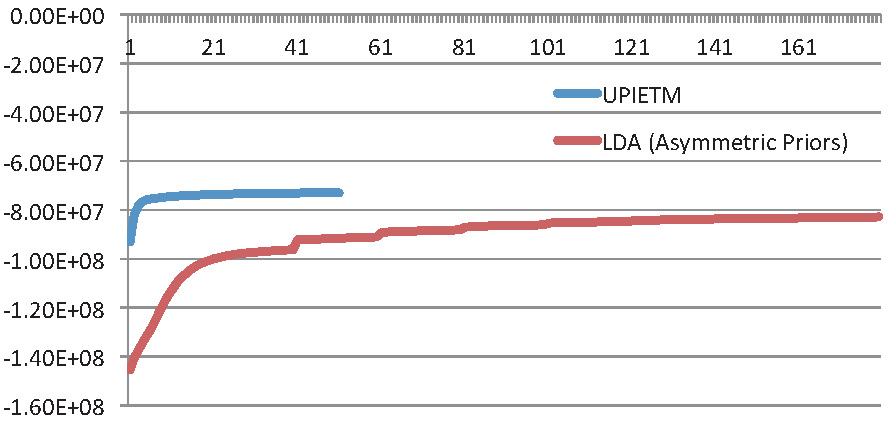
\includegraphics[height=8cm]{img/completeLoglikelihood.pdf}
        }          
        \hspace{1.5cm}
        \subfigure[Efficiency of UMIETM. x: time window, y: duration]{
                \label{fig:subfig:b} %% label for second subfigure
                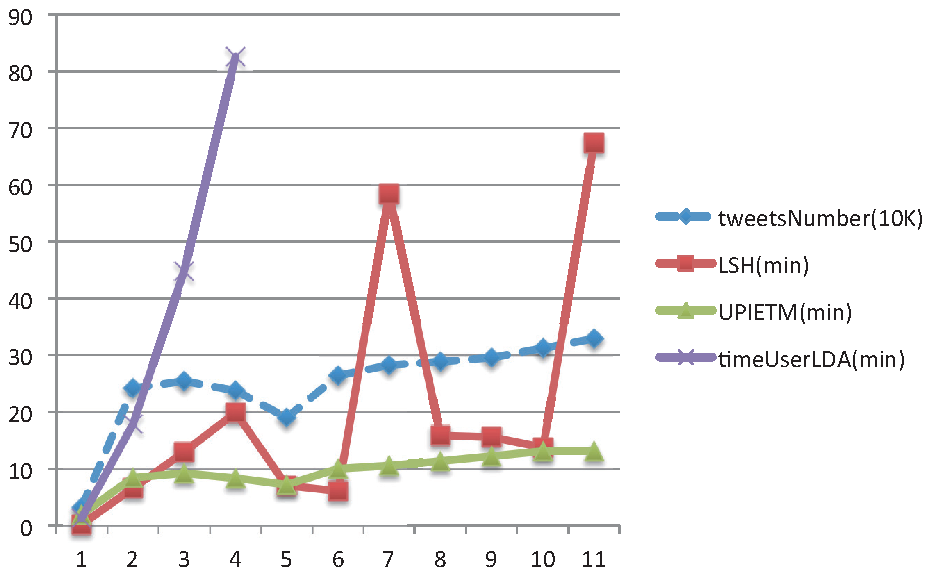
\includegraphics[height=8cm]{img/efficiencyCompareWithLSH.pdf}
        } 
%        \caption{Illustration on clustering result with different C} 
\end{figure}


\end{itemize}
\end{block}

\begin{block}{References}
\setbeamertemplate{bibliography entry author}{\vspace*{-1.25ex}\raggedright}
\setbeamercolor{bibliography entry author}{fg=black}
\setbeamerfont{bibliography entry author}{size=\small}
\setbeamertemplate{bibliography item}[text]
\begin{thebibliography}{9}
\bibitem{timeUserLDA:2012}
\footnotesize{Qiming Diao, Jing Jiang, Feida Zhu, and Ee-Peng Lim. Finding bursty topics from microblogs. In: \emph{ACL 2012}.}
\bibitem{LSH:2010}
\footnotesize{Streaming first story detection with application to twitter. In: \emph{HLT-NAACL 2010}.}
\bibitem{weng2011eventWavelet}
\footnotesize{Event Detection in Twitter. In: \emph{ICWSM 2011}.}
\end{thebibliography}
\vspace*{-1.25ex}
\end{block}
}
\end{column}

\end{columns}
\end{frame}
\end{document}
